\documentclass[border=0pt]{standalone}
\usepackage{tikz}
\usetikzlibrary{shapes.geometric, positioning, calc, decorations.pathreplacing, arrows.meta, bending}
\usepackage{amsmath}
\usepackage{pgfplots}
\pgfplotsset{compat=1.8}
\usepgflibrary{shadings}
\usepackage{xcolor}
\usepackage{microtype}
\usepackage{lmodern}

\definecolor{navyblue}{HTML}{8babf1}
\definecolor{ol}{rgb}{0.12, 0.21, 0.5}
\definecolor{oh}{rgb}{0.16, 0.63, 0.5}

\begin{document}

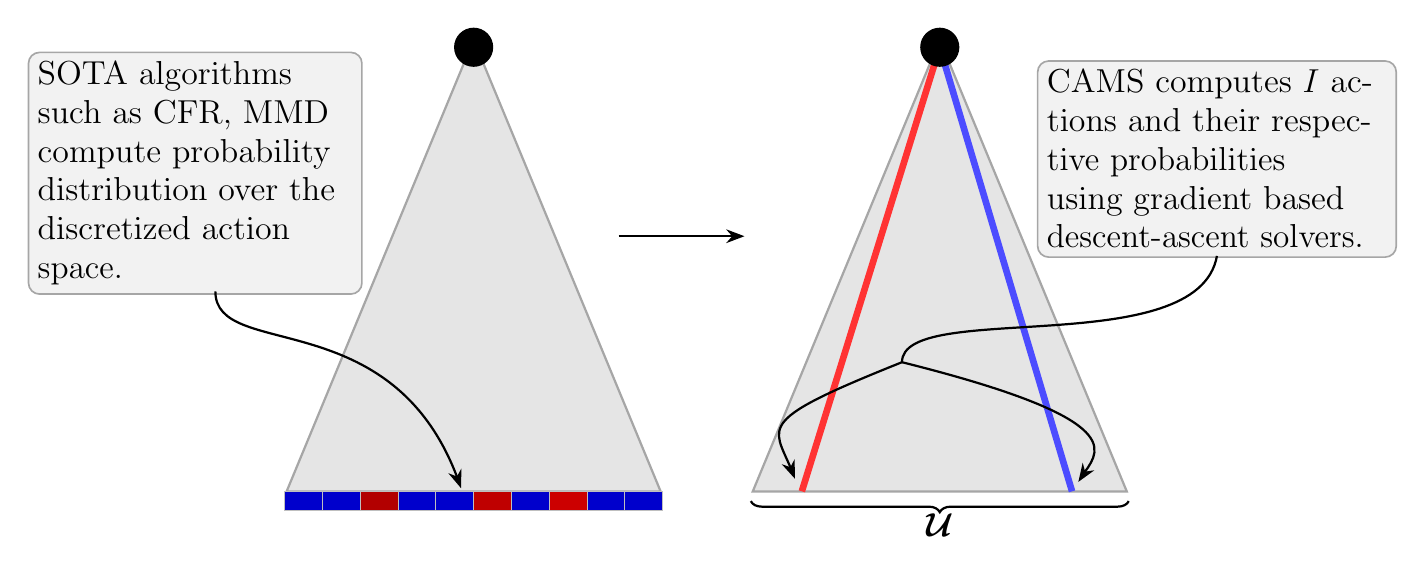
\begin{tikzpicture}[every node/.style={font=\small}]
\tikzset{every node/.style={font=\large}}

%----------------
% Left diagram
%----------------
\begin{scope}[shift={(2.08, 0)}, scale=2.4]
  % Left triangle (lighter fill, subtler line)
  \node[
    isosceles triangle, 
    rotate=90, 
    fill=gray!20,
    draw=gray!70,
    line width=0.8pt,
    minimum size=4.75cm,
    behind path
  ] (B1) at (0.2, -1.7){};

  % Probability distribution boxes
  % \foreach \i/\prob in {
  %   0/0.05, 1/0.05, 2/0.3, 3/0.25, 4/0.05,
  %   5/0.05, 6/0.05, 7/0.4, 8/0.05, 9/0.05
  % } {
  %   \pgfmathparse{\prob}\let\temp=\pgfmathresult
  %   \pgfmathparse{\temp}\let\r=\pgfmathresult
  %   % \pgfmathparse{0.7*\temp}\let\g=\pgfmathresult
  %   \pgfmathparse{0}\let\b=\pgfmathresult
  %   \definecolor{cellcolor}{rgb}{1,0,\b}
  %   \fill[cellcolor, draw=gray!50, line width=0.3pt]
  %     ({-0.8 + \i*0.2}, -2.45) rectangle ({-0.8 + (\i+1)*0.2}, -2.35);
  % }
\foreach \i in {0,...,9} {
  % Check if \i is one of the "red indices" (2, 5, 7):
  \ifnum\i=2
    \definecolor{cellcolor}{rgb}{0.7,0,0} % RED
  \else\ifnum\i=5
    \definecolor{cellcolor}{rgb}{0.75,0,0} % RED
  \else\ifnum\i=7
    \definecolor{cellcolor}{rgb}{0.8,0,0} % RED
  \else
    \definecolor{cellcolor}{rgb}{0,0,0.8} % BLUE
  \fi\fi\fi
  
  % Draw the rectangle
  \fill[cellcolor, draw=gray!50, line width=0.3pt]
    ({-0.8 + \i*0.2}, -2.45) rectangle ({-0.8 + (\i+1)*0.2}, -2.35);
}

  % Black circle at top
  \node[circle, fill=black, inner sep=5pt] at (0.2, 0){};

\end{scope}

% SOTA algorithms text box
\node[
  draw=gray!70, 
  line width=0.6pt, 
  text width=4cm, 
  rounded corners, 
  fill=gray!10
] at (-0.976,-1.6) (B1Note)
{
  SOTA algorithms such as CFR, MMD compute probability distribution over the discretized action space.
};

% Left curved arrow
\draw [line width=0.8pt, ->, >=Stealth]
  (-0.72, -3.1) .. controls (-0.72,-4) and (1.6, -3.2) .. (2.4, -5.6);

% Right arrow
\draw[->, line width=0.8pt, >=Stealth]
  (4.4, -2.4) -- (6, -2.4);

%----------------
% Right diagram
%----------------
\begin{scope}[shift={(8, 0)}, scale=2.4]
  \node[
    isosceles triangle,
    rotate=90,
    fill=gray!20,
    draw=gray!70,
    line width=0.8pt,
    minimum size=4.75cm,
    behind path
  ] (B2) at (0.2, -1.7){};

  % Chosen actions lines
  \draw[line width=2.4pt, color=red!80] (0.2, 0) -- (-0.53, -2.35);
  \draw[line width=2.4pt, color=blue!70] (0.2, 0) -- (0.9, -2.35);

  \node[circle, fill=black, inner sep=5pt] at(0.2, 0){};

  % Brace for A
  \draw [
    line width=0.8pt, 
    decorate,
    decoration={brace, amplitude=4pt, mirror, raise=3.2ex}
  ]
  (-0.8,-2.2) -- (1.2, -2.2)
  node[midway,yshift=-2.24em]{$\boldsymbol{\mathcal{U}}$};

\end{scope}

% CAMS text box
\node[
  draw=gray!70,
  line width=0.6pt,
  text width=4.32cm,
  rounded corners,
  fill=gray!10
] at (12,-1.42) (B2Note)
{
  CAMS computes $I$ actions and their respective probabilities \\
  using gradient based descent-ascent solvers.
};

% Large curved arrow on the right side
\draw [line width=0.8pt, ->, >=Stealth]
  (12, -2.65) .. controls (11.76, -4) and (8, -3.2) .. (8, -4) % main curve
  .. controls (6, -4.8) and (6.4, -4.8) .. (6.64, -5.48); % left branch

\draw [line width=0.8pt, ->, >=Stealth]
  (8, -4) .. controls (11.2, -4.8) and (10.4, -5.2) .. (10.24, -5.52); % right branch

\end{tikzpicture}

\end{document}
